\documentclass[a4paper,titlepage]{article}
\usepackage{graphicx} % Required for inserting images
\usepackage{amsmath}

\usepackage[T1]{fontenc}
\usepackage{geometry}
\usepackage{comment}
\usepackage[utf8]{inputenc}
%\usepackage[nonumberlist]{glossaries}
\usepackage[
backend=biber,
style=authoryear,
]{biblatex}
\usepackage{fancyhdr}
\usepackage{hyperref}
\usepackage{float}
\addbibresource{Bibliography.bib} %Imports bibliography file
\DeclareDelimFormat{nameyeardelim}{\addspace}
\renewcommand*{\mkbibparens}[1]{\mkbibbrackets{#1}}
\let\cite\parencite 




%glossary setup
%\makeglossaries
%\setglossarystyle{list}
%\renewcommand*{\glsnamefont}[1]{\textnormal{#1}}
%\setlength{\glsnamewidth}{\linewidth}



%add new entries here. when using them in text, use \gls

%\newglossaryentry{Coulomb Collision}{
%name=Coulomb Collision
%description = {}
%t}

%\newglossaryentry{Torr}{
    %name=Torr,
    %description={One of the many pressure units in fusion science. 1 Torr is defined as $\frac{1}{760}$ of 1 %standard atmosphere (101325kPa)}
%}
%\newglossaryentry{Divergence}{
%    name = $\nabla \cdot f$,
%    description = {Divergence operator. A vector calculus operator on a vector field $f$ }
%}
%\newglossaryentry{E-field}{
%    name = $\vec{E}$,
%    description = {Electric field vector}
%}
%\newglossaryentry{Charge Density}{
%    name = $\rho$,
%    description = {Charge Density}
%}
%\newglossaryentry{Permittivity of Free Space}{
%    name = $\epsilon_0$,
%    description = {Permittivity of free space}
%}
%\newglossaryentry{Charge State}{
%    name = $Z$,
%    description = {Species charge state}
%}





% Set different margins for each side
\geometry{top=2cm, bottom=2cm, left=2cm, right=2cm}



%title page
\title{Desktop Star in a Jar: A study of inertial electrostatic confinement fusion devices}


\author{Calvin Dai}
\date{\today}

\begin{document} 
\maketitle

\tableofcontents
\newpage
\newpage
\begin{flushleft}

\section{Definitions and Symbols}



\section{Introduction}
\label{intro}
[NOTE: NOTES ON EXPERIMENT AT THE END ARE PLANS. NOT YET DONE]

The Inertial Electrostatic Confinement (IEC) device is a unique type of fusion reactor. Conceived and developed in the 1950s and 60s by Philo T. Farnsworth in correspondence with Robert L. Hirsch(also known for his invention of the electronic television), they are unlike the much more famous and expensive tokamaks and inertial confinement systems which use magnetic fields and lasers respectively to confine fusion plasmas. Instead, IEC devices use electric fields to accelerate and confine fuel ions. They can be built for a fraction of the cost of a tokamak, with many universities and hobbyists being able to build relatively small and inexpensive units in a short period of time. \newline

Despite this financial advantage, analyses have concluded that IEC - as a physical concept - faces significant challenges before it can compete with tokamaks and laser confinement projects as viable sources of fusion power.  Inherent inefficiencies in the confinement scheme severely restrict their fusion reaction rates, which are several orders of magnitude below magnetic and laser confinement results. \cite{rider_1995_a}\cite{miley_2013_inertial} \newline

Present fusion results however allow IEC devices to occupy a useful niche in the form of highly effective neutron sources, with wide-ranging potential applications in research and industry. It also offers a platform for the study of plasma glow discharges, which are unique in that they are not thermonuclear, or, they strongly do not follow a Maxwell-Boltzmann energy distribution unlike many of the plasmas described in current plasma and fusion plasma literature.\newline 
%Unlike these plasmas, the IEC plasma is more closely resemblent (and should ideally be) of beam behaviour; an often-used alternative name is "spherically convergent ion focus" or "beam"\cite{thorson_1997_convergence} 


This paper presents a design of such a system capable of fusion, and an experimental analysis of a plasma that was generated using a significantly simplified configuration of the design to comply with institution safety regulations. The experimental configuration is not capable of fusion due to voltage safety restrictions, which therefore limits maximum ion energy.\newline 

[PLANNED] Instead, the spectrogram of the plasma is analysed at different points along the plasma to investigate the ion velocity and density to estimate the potential profile and therefore the confinement characteristics of the device. 

A simulation of the system [was] also conducted to validate the design and its results using IBSimu, an open source iterative Vlasov-Poisson ion optics library in C++ that allows for the calculation of space-charge effects from ion trajectories inside electric fields. [Model is in progress, plan is to verify experimental data from the spectrometers]


\section{Theory}
\label{theory}

\subsection{General configuration of an IEC device}
\label{general_config}

IEC devices use two either spherically or cylindrically symmetrical wire grids to produce a uniform electric field. A negative high voltage - either pulsed or steady DC - is applied across the highly-transparent central cathode grid, whilst the outer grid is earthed so that a radially inward electric field is generated towards the cathode. 
\begin{figure}[H]
    \centering
    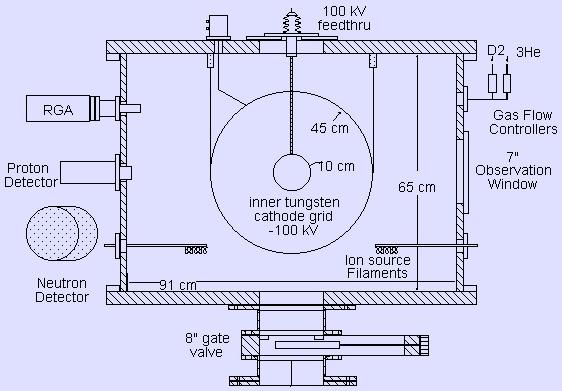
\includegraphics[width=0.5\linewidth]{iec_homer.jpg}
    \caption{Schematic of the IEC device at the University of Wisconsin-Madison, "Homer", designed to use Deuterium and Helium-3 as fusion fuel.}
    \label{fig:iec_homer}
\end{figure}

These grids are suspended on insulated feed-through stalks in the centre of a vacuum chamber, which is pumped down to pressures close to $10^-7$ Torr ($10^-5 $Pa) \cite{miley_2013_inertial} to evacuate the chamber of contaminant air particles. Fuel gas - such as deuterium is then subsequently introduced, raising the chamber pressure to tens of millitorr ($\approx 1$ Pa) before the voltage across the cathode grid is raised to several tens of kilovolts to produce a plasma discharge. 

\section{Construction overview} [body needs restructuring: current structure makes no sense]
\subsection{Vacuum}
\subsection{Safety Considerations}

\subsection{Plasma definition and characteristics}
\label{plasma_def_char}

\subsubsection{What is a plasma?}
\label{wtf_is_a_plasma_eagle_noise}
An ideal plasma is a "quasi-neutral gas of charged particles showing collective behaviour" \cite{gibbon_2014_introduction}. "Quasi-neutrality" means that although the plasma consists of non-neutral ions and electrons, the number density of positively charged ions and electrons approximately cancel out to locally balance. This can be expressed as: 

\begin{equation}
n_e \simeq Zn_i 
\end{equation}

"Collective behaviour" is the idea that the plasma's behaviour is governed predominantly by long-range macroscopic electric and magnetic fields as opposed to microscopic electrostatic and magnetic interactions between neighbouring particles in the plasma caused by the motions of each individual particle and their effects on their neighbours. Therefore we can treat its behaviour as that of a whole entity, depending on the energy distribution of the particles. If a plasma is in thermal equilibrium (i.e. described by a Maxwell-Boltzmann distribution), we can model them as fluids. 

This makes the plasma an extremely good conductor of electricity. This implies that the interior of the plasma is shielded from internal electric fields of the individual particles. \cite{freidberg_2008_plasma} \newline

The shielding effect is known as Debye shielding, which consequently leads to the definition of the Debye length scale which can quantify the degree of collective effects and therefore plasma-like behaviour in an ionised gas. 

If we place a test charge inside the ionized gas, this therefore produces a tiny perturbation in the charge density in an otherwise quasi-neutral environment. As a result of Gauss' law for electrostatics:

\begin{equation}
\nabla \cdot \vec{E} = \frac{\rho}{\epsilon_0}
\end{equation}
a net electric field arises, exerting a force on neighbouring charges.

Like charged particles (ions) are repelled away and oppositely charged particles (electrons) are attracted towards the test charge. Since the mass of an electron is much smaller than the mass of an ion, on the timescale of the electron's motion we can assume that the ions are motionless.

As they accelerate towards the test charge, eventually the $\vec{E}$ = 0. However, due to the inertia of the charges they overshoot to form another region of net charge density, and this oscillatory pattern repeats, known as a Langmuir wave. The frequency of these oscillations is given by the Bohm-Gross dispersion relation, which can be expressed as:

\begin{equation}
    \omega=\sqrt{\frac{e^2n_{0}}{\epsilon_0 m_e} + 3k^2 v_{th, e}^2}
\end{equation}

where k is the wave number and $n_0$ is the initial number density of electrons before the test charge is introduced. The first term is the fundamental plasma frequency, derived from a fluid model of the oscillations in a cold plasma, and the second term is a thermal correction factor, generalising the expression for a finite-temperature plasma \cite{mcgreivy_2024_general}. \newline

To further justify the stationary condition of the ions, we can similarly compute the (singularly charged) ion frequency of oscillation, replacing $m_e$ with $m_i$. If we ignore the thermal correction factor (i.e. consider a cold plasma) the ratio of $\omega_e$ to $\omega_i$ is therefore $\sqrt{\frac{m_i}{m_e}}$. For fuel plasmas such as deuterium where Z = 1, this ratio is ~ 60. On the timescale of an electron's oscillation, an ion is therefore approximately stationary. 

As the electrons keep oscillating, they gradually thermalise to equilibrium due to energy losses from small-angle Coulomb scattering between the ions.
The overall effect is that the extra potential from the test charge is equalised and the plasma maintains its quasi-neutrality. 
\begin{figure}[H]
    \centering
    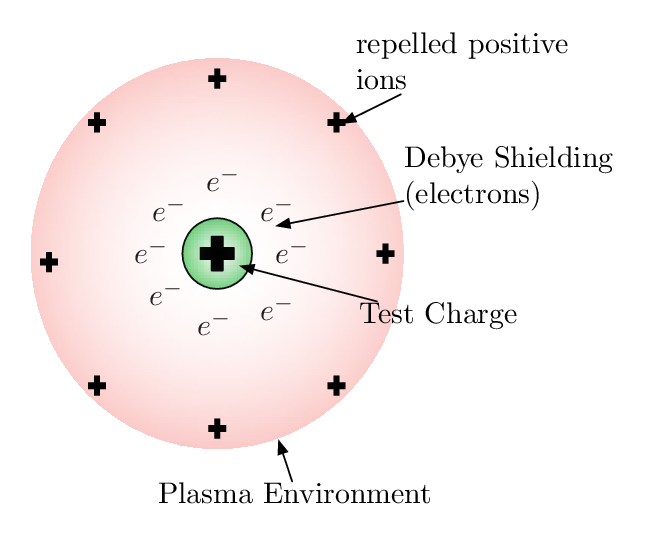
\includegraphics[width=0.5\linewidth]{debye shielding.png}
    \caption{Illustration of Debye Shielding \cite{Coulomb_thrusting_debye}}
    \label{fig:debyeshielding}
\end{figure}

Once at equilibrium , the Debye length can be interpreted as the distance over which the electric potential from the test charge decreases by a factor of $\frac{1}{e}$ ($\approx$ 37\%). It is expressed as 

\begin{equation}
\lambda_d = \sqrt{\frac{\epsilon_0 k_B T_e}{e^2 n_e}}
\end{equation}

This expression relies on the assumption that the energy distribution of the electrons follows a Maxwell-Boltzmann probability distribution. \cite{freidberg_2008_plasma}. Although it is a unique property of IEC devices that their energy distributions in operation are highly non-Maxwellian, Godyak et al. found that in the initial phase of the formation of helium and argon glow discharge plasmas (see section~\ref{discharge_iecplasma_form}), the electron energy distribution function becomes Maxwellian \cite{godyak_1992_evolution}. It would be reasonable to assume that a similar phenomenon would occur for other fuel gases such as deuterium. 

We can also calculate the number of particles in a Debye sphere, i.e. a sphere of radius $\lambda_d$:

\begin{equation}
    N_D = n\frac{4}{3}\pi\lambda_D^3
    \label{plasma_param}
\end{equation}

The condition for collective behaviour is known as the plasma parameter, or:
\begin{equation}
    N_D \gg 1
\end{equation}
\cite{chen_2016_introduction} \cite{freidberg_2008_plasma}
This means that the density of particles must be sufficiently high for a ionized gas to be classed as a plasma.


\subsubsection{How does a plasma form in an IEC device?}
\label{discharge_iecplasma_form}

In IEC devices, the plasma forms through the electric breakdown of the fuel gas into a glow discharge. Breakdown occurs when a strong enough electric field is applied across a gap. 

This is because any gas will contain stray ionized particles and electrons. This is due to random ionization of gas molecules by cosmic rays, background radiation and ultraviolet light in a process analogous to the photoelectric effect in metals. If a potential is applied between two cathodes in the gas, an electric field is produced and therefore the charges are accelerated: ions towards the cathode, electrons towards the anode. The electrons initially accelerate to higher velocities faster, as they are lighter than the ions, quickly accelerating to energies higher than the ionization threshold of the neutral gas molecules, ionizing them. This produces further ions and electrons, which each then also move to the cathode and anode respectively; the latter ionize more ions and the cycle repeats in an exponential process known as the Townsend avalanche. \newline

\begin{figure}[H]
    \centering
    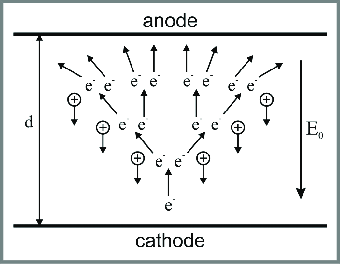
\includegraphics[width=0.5\linewidth]{Townsend-breakdown-and-electron-avalanche-formation-between-two-electrodes-Adapted-from.png}
    \caption{Townsend Avalanche \cite{ollegott_2020_fundamental}}
    \label{fig:townsend}
\end{figure}

Paschen's law states that the voltage at which this breakdown occurs is a function of pressure and gap distance between the electrodes, and certain breakdown characteristics and constants of the gas occupying the electrode gap. \cite{fu_2020_discharge}Experimental measurements of this voltage at different pd values forgive curves known as Paschen curves. 

\begin{figure}[H]
    \centering
    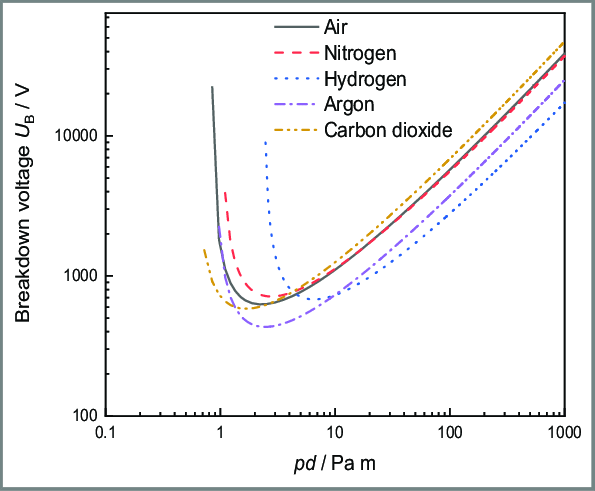
\includegraphics[width=0.5\linewidth]{Breakdown-Paschen-curves-for-different-gases-The-data-is-plotted-with-Paschen.png}
    \caption{Paschen curves for different gases \cite{ollegott_2020_fundamental}}
    \label{fig:paschen}
\end{figure}

Assuming a fixed volume, as pressure decreases (left side of the "V" curve), the electric potential required to induce an avalanche grows extremely quickly, due to the low density of particles. This means that when "seed electrons" \cite{raizer_1991_gas} from random ionization are accelerated by the field, they have an extremely long mean free path that means the likelihood that they actually collide and ionize a background neutral molecule is very low. To compensate for this, the energy per collision must be extremely high to increase the impact ionization cross section (see section~\ref{cross_section}) for the greatest likelihood of successful ionization.

Similarly if the gap distance is very low, then the electrons will not be able to accelerate to high enough energies to induce significant ionization before they are lost to the grounded anode, thus a much higher field strength is required to compensate. 

At the low operating pressure of IEC devices ($\approx1$ Pa), the discharge regime is firmly on the left side of the Paschen "V" shape, meaning that the discharge requires a high operating voltage to be sustained. 

In this breakdown regime, we are still considering the individual motions of each particle. The density of charges is not high enough for collective behaviour to satisfy the plasma parameter. Eventually, as the avalanche continues, and the electron current through the discharge increases, we transition to the next regime along the DC discharge I-V graph: [rubbish explanation- fix]

\begin{figure}[H]
    \centering
    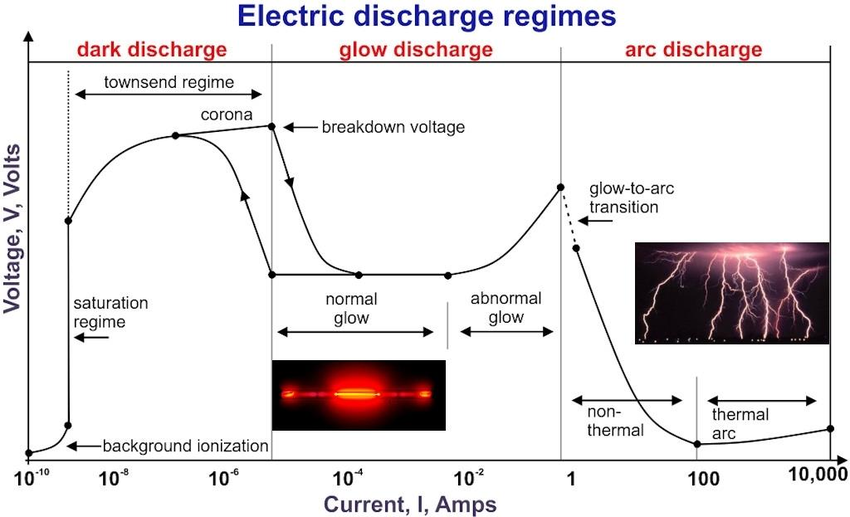
\includegraphics[width=0.5\linewidth]{An-overview-of-the-different-electric-discharge-regimes-possible-86.png}
    \caption{DC discharge regime I-V cruve}
    \label{fig:discharge_regimes}
\end{figure}

which is our glow discharge. 

[need to talk about normal -> abnormal glow, initial sheaths, mean free path lengthening to enter glow regimes: glow, jet, star modes]


[also rubbish and incomplete. Liebermann and Lichtenberg. mean free path etc.]




\subsection{How are plasma particles confined?}
\label{confinement}

In the ideal case for maximum fusion rate, all of the ions in an IEC device are born at maximum energy and will be trapped - or confined - in an electrostatic potential well inside the system. 

Before the fuel is introduced to the chamber, a single spherically symmetrical potential well profile is present.

\begin{figure}[H]
    \centering
    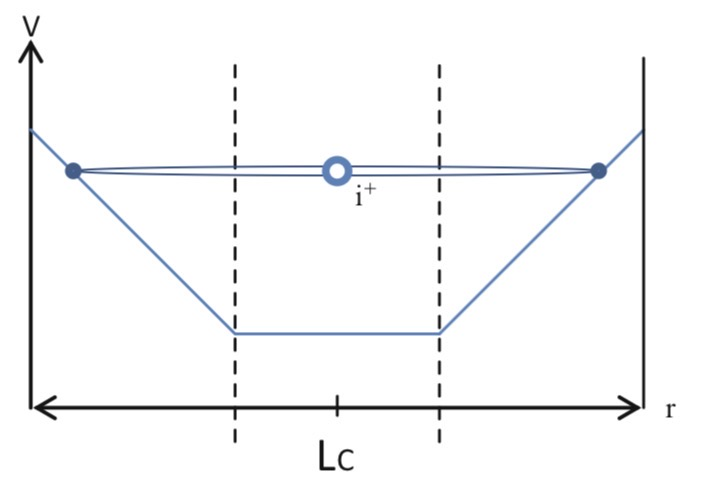
\includegraphics[width=0.5\linewidth]{simplepotential.jpg}
    \caption{Linear Potential Profile of IEC device at low ion current and no space charge effects(plot own with matlab later) \cite{miley_2013_inertial}}
    \label{fig:linear_pot}
\end{figure}

Once we introduce fuel molecules into the system, our discharge process begins. The maximum energy a seed electron can have in the system must be equal to the product of $e$ and the cathode potential $V$, and therefore following ionisation - depending on where the ion is born and the potential $\phi$ at that point - it's maximum energy must also be equal to $e\phi$. The ions fall towards the negative cathode before (ideally) passing through the grid openings and then entering the oscillatory recirculations introduced in section~\ref{general_config}. To maximise the energy the ions can be accelerated to, fuel ions rather than neutrals are often first injected into the system so that they can be accelerated as soon as they pass through the anode grid openings. 

As the ion charge density increases and the plasma parameter (equation~\ref{plasma_param}) is satisfied, we now have an energy distribution of charges occupying the system. This distribution has its own electric field which disrupts the external field provided by the electrodes. We have now entered the space charge regime, where the potential profile of the environment is strongly influenced by the self field of the charge distribution inside the device. \cite{ferrario_2013_space_charge} \newline

A simplified model of the confinement scheme will assume the following:

\begin{itemize}
    \item The particles are non-relativistic
    \item There is no magnetic field. 
    \item There are no collisional effects between particles. This includes inter-particle Coulomb reactions and unfortunately, fusion reactions, which are the least likely inter-particle reactions in a fusion plasma. Physically this is a valid approximation given the collective behaviour of the plasma and is a common assumption. \cite{freidberg_2008_plasma} 
    [also no electrons?]
\end{itemize}

We start by importing the reactor geometry (cathode/anode grids and their potentials) and computing the electric field and potential profile with no charge in the system (giving a profile similar to Figure 6). This is due to the self-consistent nature of the system: a change in charge density changes the potential profile, which then changes the charge density again etc. The potential at each point can be solved by Poisson's equation for electrostatics: 

\begin{equation}
    \nabla^2\phi = -\frac{\rho}{\epsilon_0}
    \label{poisson}
\end{equation} 

and so in the zero-charge limit this simplifies to Laplace's equation:

\begin{equation}
    \nabla^2\phi = 0
\end{equation} 

%The Laplacian operator of the potential can be interpreted as the difference between the potential at that point with the average potential of the its surroundings. 
We can then computationally introduce a population of particles into the system, and compute their trajectories to find their positions and velocities as functions of time. 

To find the charge density at a certain point in the system, we must consider the overall behaviour of the system using a smooth distribution function. This is a 6 dimensional time-evolving probability density distribution of particles at positions $\vec{r}$, velocities $\vec{v}$ and time $t$:

\begin{equation}
    f(\vec{r}, \vec{v}, t)
\end{equation}

To find the equilibrium state of the self-field and external field interaction, we set the time derivative of the distribution function to 0. Expanding into partial derivatives using the chain rule and substituting $\frac{\partial \vec{v}}{\partial t} = \frac{q}{m}\vec{E}$ yields the Vlasov-Poisson equation:

\begin{equation}
    \frac{\partial f}{\partial t} +\vec{v} \cdot \frac{\partial f}{\partial \vec{r}} + \frac{\partial f}{\partial v} \cdot \frac{q}{m}\vec{E} = 0
\end{equation}

We can then calculate the charge density at each point of the system  by taking the integral of the distribution function with respect to $\vec{v}$ (giving the number density) and multiplying by the total charge in the system:

\begin{equation}
    \rho(t) = Q_{tot} \int f(\vec{r}, \vec{v}, t) d^3v
\end{equation}

The potential profile can then be computed using Poisson's equation. To find the equilibrium state of the potential profile we must iterate this process until convergence.
[Need to also consider plasma sheathing and shielding at grid wires. this also only currently talks ions; electrons very important]

A flow diagram for the program is as follows:
\begin{figure}[H]
    \centering
    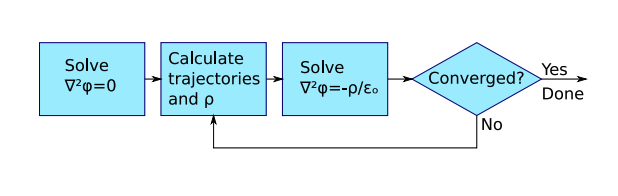
\includegraphics[width=0.5\linewidth]{ibsimuflow.png}
    \caption{Flow diagram for confinement simulation. Source: T. Kalvas https://ibsimu.sourceforge.net/jss2015/introduction.pdf}
    \label{fig:vlasov iteration}
\end{figure}

The ion optics software library IBSimu (Ion Beam Simulator) was chosen as it follows this exact iterative cycle. Originally developed for ion beam extraction simulations for particle accelerators, IBSimu takes into account all relevant processes in an IEC confinement system: the 3D computation of $\vec{E}$ fields with imported geometries, space charge effects, and plasma sheathing effects at electrode boundaries. \cite{tkalvas_2010_scpibsimuscp}. 




\subsection{How does Fusion occur?}
\label{fusion}

\subsubsection{Fusion reactions} 
\label{fusion_reactions}



Typical IEC devices utilise fuels consisting either of pure deuterium or deuterium-tritium mixes. The deuterium-deuterium (D-D) reaction has two pathways with a roughly equal chance of occurence:

\begin{equation*}
{}^{2}_{1}\mathrm{H} + {}^{2}_{1}\mathrm{H}
\rightarrow
{}^{3}_{2}\mathrm{He} + {}^{1}_{0}\mathrm{n}
\quad (Q = 3.27\,\text{MeV})
\end{equation*}

\begin{equation*}
{}^{2}_{1}\mathrm{H} + {}^{2}_{1}\mathrm{H}
\rightarrow
{}^{3}_{1}\mathrm{T} + {}^{1}_{1}\mathrm{p}
\quad (Q = 4.03\,\text{MeV})
\end{equation*}

and for the deuterium-tritium (D-T) reaction:

\begin{equation*}
{}^{2}_{1}\mathrm{H} + {}^{3}_{1}\mathrm{T}
\rightarrow
{}^{4}_{2}\mathrm{He} + {}^{1}_{0}\mathrm{n}
\quad (Q = 17.6\,\text{MeV})
\end{equation*}

The energy gains (calculated from the binding energy difference between the reactancts and the products) show that the D-T reaction is far more favourable compared to the D-D reaction from an energy production perspective. 

In a realistic IEC device, the reactions are more complex. This is due to the fact that not all of the neutral deuterium molecules are ionized following introduction to the reaction vessel. Many ions will also lodge themselves into the metal lattice of the anode and cathode grid wires and the chamber walls. In their investigation of a pulsed cylindrical IEC device - which holds the world record for overall neutron production rate - Tomiyasu et al. identified seven reaction regimes (which are still applicable to spherical and other shapes of device):

\begin{itemize}
    \item Beam-beam (BM-BM): Occurs between ions in the star-mode beams. This is the ideal scenario to reduce energy loss from collisions with the grid wires, the main limiting factor to IEC reaction rate. 
    \item Beam-background (BM-BG): Occurs between beam ions and background neutrals in the chamber which are not circulating through the beams. 
    \item Beam-Cathode (BM-C): Occurs between beam ions and ions that become lodged into the cathode grid wires.
    \item Fast neutral-background (CX-BG): if an ion collides with a background neutral, there is a probability (quantified by the charge-exchange cross section) that the ion acquires an electron from the neutral, and the neutral therefore gains the charge of an ion. The former ion is now a high-energy neutral atom experiencing no force from the electric field of the system, moving at a constant velocity through the chamber until it collides and fuses with another background neutral.
    \item Fast neutral - cathode (CX-C): The high-energy neutral now collides with a lodged ion in the cathode grid wires.
    \item Fast neutral - anode (CX-A): ditto for anode grid wires
    \item Fast neutral - chamber wall (CX-W): ditto for chamber walls. 
\end{itemize}


However, even the IEC device with the highest ever recorded neutron production rate (and therefore highest reaction rate) has the lowest yield from beam-beam reactions. In fact, the reactor with the world record for neutron production rate (NPR) - and therefore fusion rate \cite{tomiyasu_2009_effects} had BM-BM as the lowest contributor to the overall production rate by over five orders of magnitude. The dominant reaction regimes were BM-C and BM-BG. This highlights  one of the fatal inefficiences of an IEC device caused by presence of the grid wires. 

\subsubsection{How likely is fusion?}
\label{cross_section}

The probability of a nuclear reaction occuring between these species is characterised by a quantity called the cross section. If we consider two colliding particles, the cross section can be interpreted as the circular area (measured in barns = $10^{-28} \text{ m}^2$ projected from the target particle normal to the velocity of the incident particle. If the incident particle passes through this area with sufficient energy, then the force exerted on the target particle is sufficient to overcome the Coulomb repulsion between them for the nuclear reaction to occur. The cross section is therefore a function of the energy of the incident particle relative to the target particle (many reactions and kinetic processes have cross sections, including for collisional ionization, as referenced in section~\ref{discharge_iecplasma_form}).

Quantum mechanical effects of tunnelling and resonance also have to be taken into account to give an accurate model of the reaction probability at different energies. 

\begin{figure}[H]
    \centering
    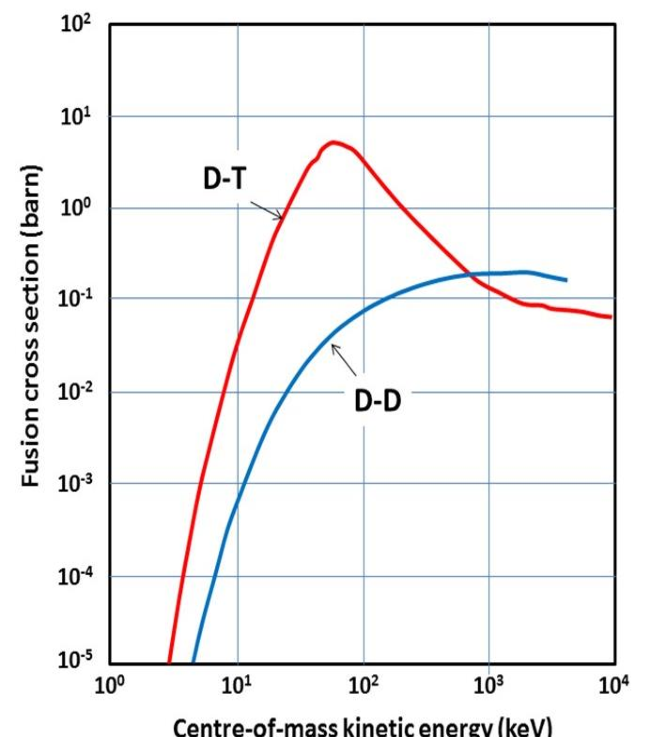
\includegraphics[width=0.5\linewidth]{Cross-sections-for-the-neutron-producing-D-D-and-D-T-nuclear-fusion-reactions-as-a.png}
    \caption{Cross Section Data for D-D and D-T reactions as a function of incident particle energy in the incident frame.\cite{bjrnstad_2021_modern}}
    \label{fig:placeholder}
\end{figure}
Figure 3 shows that the D-T reaction is far more favourable; its resonance peak of around 5-6 barns at around 50-60keV is two orders of magnitude higher than for D-D.






\subsection{Numerical model of confinement in the experimental setup}

\subsubsection{Historical Overview of Numerical Methods}

[mention difficulty in simulating the device due to many random factors, difficulty to probe plasma without perturbation etc]
Prior studies into the potential profiles of spherical IEC devices have shown that convergence of ions in the centre of the cathode grid forma into a dense core, the positive space charge density increases the potential at the centre of the and therefore central "virtual anode" structures form. If multiple of these structures form, then deep internal potential well structures can form inside the core of the device, providing a dense core region where fusion can occur efficiently. 

There have been conflicting claims in the literature about the formation of so-called "well within a well" or "double potential well" structures, as shown in the figure below:

\begin{figure}[H]
    \centering
    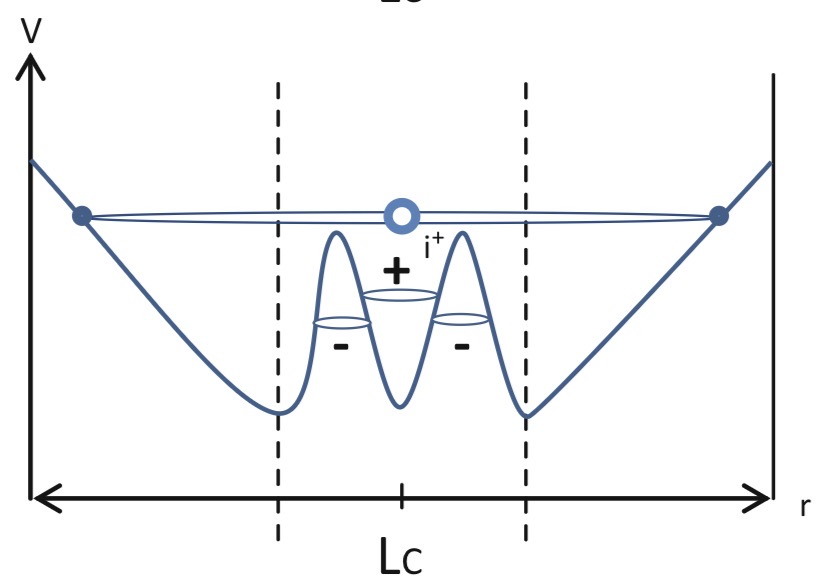
\includegraphics[width=0.5\linewidth]{IMG_1100.jpg}
    \caption{Double Potential Well Structure}
    \label{fig:double_well}
\end{figure}

Gu and Miley have addressed issues with prior experiments and provide new data through improved spacial resolution of measurements to verify that double potential well structures do indeed form in certain configurations of IEC devices \cite{gu_2000_experimental}, verifying the initial ground-breaking work in the field made by Hirsch in 1967 \cite{hirsch_1967_inertialelectrostatic}









\newpage

\printbibliography

\end{flushleft}
\end{document}
